\subsection{Herausforderungen}

Bei der Implementierung der Funktionen des Volksbot traten einige Herausforderungen auf, deren Lösungen besonderen Aufwand hervorriefen oder nicht umgesetzt wurden. Ein Beispiel dafür ist die Selbstlokalisation des Roboters durch die Odometrieberechnung und dessen Verbesserung durch die adaptive Monte Carlo Lokalisation (AMCL). Aufgrund der Fehleranfälligkeit der einfachen Odometrie durch Einflüsse wie z.B. die Beschaffenheit des Bodens ist der Einsatz von Algorithmen wie die adaptive Monte Carlo Lokalisation, welcher die Daten des Laserscanners nutzt, notwendig.  Die Qualität der Odometrie musste durch das Kalibrieren des Parameters der Achsenlänge des Roboters erhöht werden, um die nötige Voraussetzung für einen funktionierenden AMCL-Algorithmus zu schaffen. Eine gute Odometrie lässt sich dadurch erkennen, dass die Punkte des Laserscans auch bei Bewegung weiterhin mit den Wänden der Umgebungskarte übereinstimmen. Getestet wurde die Odometrie durch die verzögerte Darstellung der Laserscans in Rviz bei der Drehung des Roboters. Die Laserscan-Punkte würden bei einer guten Odometrie den Raum relativ genau nachzeichnen und die Laserpunkte würden sich überlappen. Ein Vergleich zwischen einer guten Odometrie-Einstellung (links) und einer schlechten (rechts) ist in Abbildung \ref{fig:Odo_vergleich} dargestellt.

\begin{figure}[h!]
 \centering
		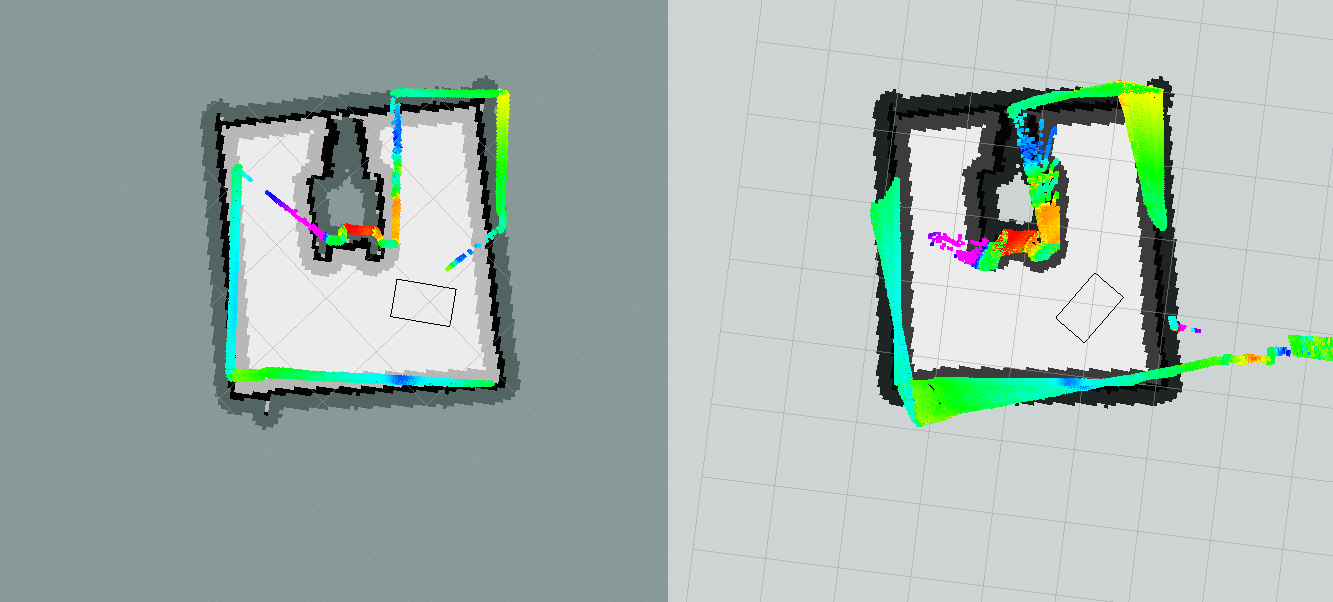
\includegraphics[width=1\textwidth]{drive/Odometrie_vergleich.png}
	\caption{Vergleich von Odometrie-Einstellungen mit Hilfe von verzögert dargestellten Laserscan-Punkten}
	\label{fig:Odo_vergleich}
\end{figure}

Bei der Parametrisierung der Wegplanung musste ein Gleichgewicht zwischen Geschwindigkeit und Genauigkeit gefunden werden, um ein stabiles System zu schaffen. Durch die Vielzahl der Möglichkeiten war die Suche nach geeigneten Einstellungen problematisch. Ein Beispiel dafür ist die Parametrisierung der Zieltoleranzen. Einerseits hat die Verringerung der Zieltoleranzen bewirkt, dass sich der Roboter der Zielposition exakter nähert. Andererseits dauert die Ausrichtung des Roboters deutlich länger, da der Roboter mehrere Rotationen ausführt bis die geeignete Position erreicht wurde. Letztlich wurde eine genauere Positionstreue des Roboters priorisiert, um die Fehleranfälligkeit bei der Paketübergabe zu senken.

Eine weitere Herausforderung stellte die Erkennung von Hindernissen dar, die ober- oder unterhalb des Laserscanners in den Raum ragen. Zur Lösung dieses Problems könnte ein weiterer bildgebender Sensor genutzt werden, um den gesamten Raum nach potenziellen Hindernissen zu untersuchen oder eine Anpassung der Arbeitsumgebung durchgeführt werden.

Mit großem Aufwand war die korrekte Ansteuerung der Maxon Controller verbunden. Besonders die Parametrisierung des kleineren Maxon Controllers unter ROS, welcher für den Betrieb des Förderbandes verwendet wird, stellte sich als Problem heraus. Schon kleinere Abweichungen der Parameter für Spannungs- und Beschleunigungswerte in der Ansteuerung des Controllers führten zu Systemabstürzen.
 
Die Programmierung und Parametrisierung der Teilfunktionen musste mit Blick auf
die CPU-Auslastung der Steuereinheit geschehen, da einige Berechnungen bei falscher
Verwendung zu sehr hohen Auslastungen und einer unzureichenden Performance des
Roboters führten. Ein Beispiel dafür ist die Funktion zur Kommunikation mit Hilfe des MICAz-Moduls, welche     regelmäßig unterbrochen werden musste.

Ein weiteres Problem stellte der LMS 100 Laserscanner von SICK dar. Dieser wird mittels Ethernet-Anschluss mit der Steuereinheit verbunden und sollte mittels seiner IP Adresse durch ROS direkt verwendet werden können. Allerdings konnte weder ROS noch SOPAS ET ( siehe Kapitel 3..3.3 ) auf den Scanner zugreifen. Beim erstellen eines Projekts in SOPAS war der Netzwerkscanassistent nicht in der Lage den Laserscanner zu erkennen und somit musste der LMS 100 manuell im Gerätekatalog ausgewählt und in das Projekt eingebunden werden. Bei der Verbindung zum LMS 100 wurde die bestehende IP Adresse des Scanners angezeigt und eine Neuzuweisung einer IP Adresse angeboten. Die Neuzuweisung der IP Adresse ist notwending, damit ROS eine Verbindung zum LMS 100 herstellen konnte.